% Figure 1 of the JORS metapaper: verification workflow of quantum-group.
% Original figure made for this paper (drafted with AI assistance; see the
% paper's generative-AI statement). Build with:  pdflatex figure1_workflow.tex
\documentclass[border=4pt]{standalone}
\usepackage[T1]{fontenc}
\usepackage{lmodern}
\usepackage{amsmath,amssymb}
\usepackage{tikz}
\usetikzlibrary{arrows.meta,positioning,calc}
\newcommand{\api}[1]{\\[3pt]\parbox{4.45cm}{\centering\ttfamily\scriptsize
  \linespread{1.0}\selectfont #1}}
\begin{document}
\sffamily
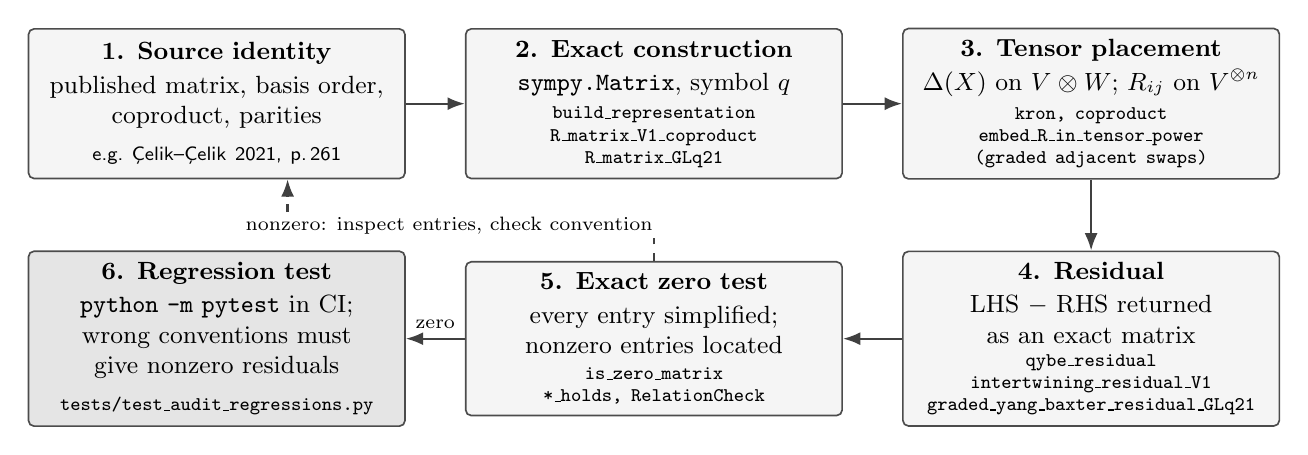
\begin{tikzpicture}[
  box/.style={draw=black!70, rounded corners=2pt, line width=0.6pt,
              fill=#1, align=center, text width=4.5cm, minimum height=1.9cm,
              inner sep=4pt, font=\small},
  box/.default=black!4,
  arr/.style={-{Latex[length=2.2mm]}, line width=0.8pt, draw=black!75},
  node distance=0.9cm and 0.75cm]

\node[box] (src) {\textbf{1. Source identity}\\[1pt]
  published matrix, basis order,\\ coproduct, parities
  \api{\sffamily e.g.\ Çelik--Çelik 2021, p.\,261}};
\node[box, right=of src] (build) {\textbf{2. Exact construction}\\[1pt]
  \texttt{sympy.Matrix}, symbol $q$
  \api{build\_representation\\ R\_matrix\_V1\_coproduct\\ R\_matrix\_GLq21}};
\node[box, right=of build] (embed) {\textbf{3. Tensor placement}\\[1pt]
  $\Delta(X)$ on $V\otimes W$; $R_{ij}$ on $V^{\otimes n}$
  \api{kron, coproduct\\ embed\_R\_in\_tensor\_power\\ (graded adjacent swaps)}};

\node[box, below=of embed] (res) {\textbf{4. Residual}\\[1pt]
  LHS $-$ RHS returned\\ as an exact matrix
  \api{qybe\_residual\\ intertwining\_residual\_V1\\ graded\_yang\_baxter\_residual\_GLq21}};
\node[box, left=of res] (zero) {\textbf{5. Exact zero test}\\[1pt]
  every entry simplified;\\ nonzero entries located
  \api{is\_zero\_matrix\\ *\_holds, RelationCheck}};
\node[box=black!10, left=of zero] (test) {\textbf{6. Regression test}\\[1pt]
  \texttt{python -m pytest} in CI;\\ wrong conventions must\\ give nonzero residuals
  \api{tests/test\_audit\_regressions.py}};

\draw[arr] (src) -- (build);
\draw[arr] (build) -- (embed);
\draw[arr] (embed) -- (res);
\draw[arr] (res) -- (zero);
\draw[arr] (zero) -- node[above, font=\scriptsize] {zero} (test);
\draw[arr, dashed] (zero.north) -- ++(0,0.45) -| ($(src.south)+(0.9,0)$);
\node[font=\scriptsize, fill=white, inner sep=1.5pt]
  at ($(zero.north)+(-2.6,0.45)$) {nonzero: inspect entries, check convention};
\end{tikzpicture}
\end{document}
